\subsection{Turing machines}

One may informally define an algorithm as a collection of simple instructions for carrying out some task. \textcite{turingComputableNumbersApplication1936} introduced the now ubiquitous model of computation. We will not bother ourselves with the granular detail of the definition of a Turing machine, as many variants exist that are all equivalent. 

\begin{theorem}[\textcite{turingComputableNumbersApplication1936}] \label{the:church-turing}
    The intuitive notion of an algorithm is equivalent to the mathematical concept of an algorithm defined by Turing machines.
\end{theorem}
% Maybe just use the previously written content about Turing machines..
A Turing machine $M$ consists of the following components:
\begin{itemize}
    \item a finite set of states;
    \item an infinite tape with storage cells, with cells containing a single symbol from some alphabet $\Pi$;
    \item a device called the head that can read and write on a cell, and move along the tape; and 
    \item a transition function.
\end{itemize}
$M$ will start its computation at an initial state, with an input on the tape, and the head at the start of the input. The head will read the contents of the cell, and by also considering the state, use the transition function to decide what to write on the cell, whether to move right or left along the tape, and what state to enter. The Turing machine will run until its enters a halt state (although it may also run forever), and the output of the machine will be the contents of the cells on the tape when the machine halts. We denote the output of a Turing machine on input $x \in \Sigma^*$ ($\Sigma \subset \Pi$ is the \emph{input alphabet}) as $M(x)$ (note this may be undefined if the Turing machine does not halt). See Figure \ref{fig:turing-machine} for a schematic of a Turing machine.

\begin{figure}
    \centering
    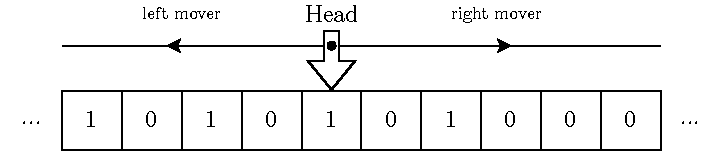
\includegraphics[width=0.8\textwidth]{content/3-complexity/images/turing-machine}
    \caption{Schematic of a Turing machine.}
    \label{fig:turing-machine}
\end{figure}

For decision problems, we disregard the machine's output but introduce two new halt states: an accept state and a reject state. If $M$ halts on input $x$ in the accept state, we say that $M$ \emph{accepts} $x$ and similarly for $M$ rejecting $x$. We denote $L(M)$ as the language of strings that $M$ accepts. If there is a Turing machine $M$ such that $\mathcal L = L(M)$, then the language $L$ is said to be \emph{semidecidable}. We say a language is \emph{decidable} if it is semidecidable and rejects all strings outside of the language.

Decision problems offer a simple introduction to modelling computation, but most of the problems we will look at expect an answer more than just \emph{yes} or \emph{no}.


We take a brief moment to comment on the existence on \emph{undecidable} problems; that is, a problem for which no algorithm decides it. 

\begin{problem}[HaltingProblem]
    Instance: let $M$ be a Turing machine and $x \in \Sigma^*$ an input. \\
    Question: does $M$ halt on $x$?
\end{problem}

\begin{theorem}
    There is no Turing machine that decides \textsc{HaltingProblem}.
\end{theorem}

\begin{proof}[Sketch of proof.]
    We omit the details of the proof, as it requires some constructs that are of little use in our context, but we provide a rough outline. We construct an adversary Turing machine $D$ that takes as input a Turing machine $M$. $D$ will accept if $M$ rejects with itself (or rather, an encoding of itself) as input. If $M$ accepts itself, then $D$ loops indefinitely. By considering how $D$ runs on the encoding of itself, we find a contradiction.
\end{proof}
